%\documentclass[12pt, tcd-mai]{mai}
\documentclass[11pt, a4paper]{article}
\usepackage{rminterim}
\usepackage{amsmath}
\usepackage{caption}
\begin{document}
% Your project title etc goes here
\title{\textbf{\textsc{\Huge Click Removal in Degraded Audio}}\\ {\Large Report for Module EEP55C22 Computational Methods}}
\author{Changhong Li, Student ID 23333239 \\ Trinity College Dublin \\ {\tt lic9@tcd.ie}}
%\address{Interim Report}

\date{October 2023}

\maketitle

\begin{center}
\begin{minipage}[t]{0.75\linewidth}
\textit{
This report is submitted in part fulfilment for the assessment required in EEP55C22 Computational Methods.  I have read and I understand the plagiarism provisions in the General Regulations of the University Calendar for the current year. These are found in Parts II and III at \myhref{http://www.tcd.ie/calendar}{ http://www.tcd.ie/calendar}.}
\end{minipage}
\end{center}

This report describes the algorithm designed for detection and removal of clicks in archived audio tracks. An example of a few clicks is shown in Figure \ref{fig1}.Clicks are like sudden, irrational spike in a waveform. The sound manifests as a short sharp click or thump in the audio track. These degradation arise because of noise in the degraded signal which maybe caused by the enviroment or something else. Our problem is to find out a model which could remove the clicks in the degraded signal and make the output signal more smooth.




\section{Background}
Let us define the observed degraded signal as $G_k$ and the original, clean signal as $y_k$. 
We can model the degradation as follows.
\begin{equation}
  G_k = \begin{cases}{cc}
              r_k & \text{when $b_k == 0$} \\
              y_k & \text{Otherwise}
              \end{cases}
\end{equation}
 where $r_k$ is a random corruption generated with rand function as clicks array which have random locations and amplitude, and $b_k$ is an indicator binary variable that is 1 at sites that are corrupted. Therefore the observed signal is created by corrupting specific sites indicated by $b_k == 1$, hence clicks shown in Figure \ref{fig2}.
      
 Our problem is to train a model using the degraded signal which could predict how it should be, and then calculate the error between degraded signal and predicted one then set up a threshold to judge if we should replace the data point with interpolation. After the correction, we will get a much more smooth signal and remove the clicks in the degraded signal.
 
\begin{figure}[htbp]
 	\centering
 	\begin{minipage}[t]{0.48\textwidth}
 		\centering
 		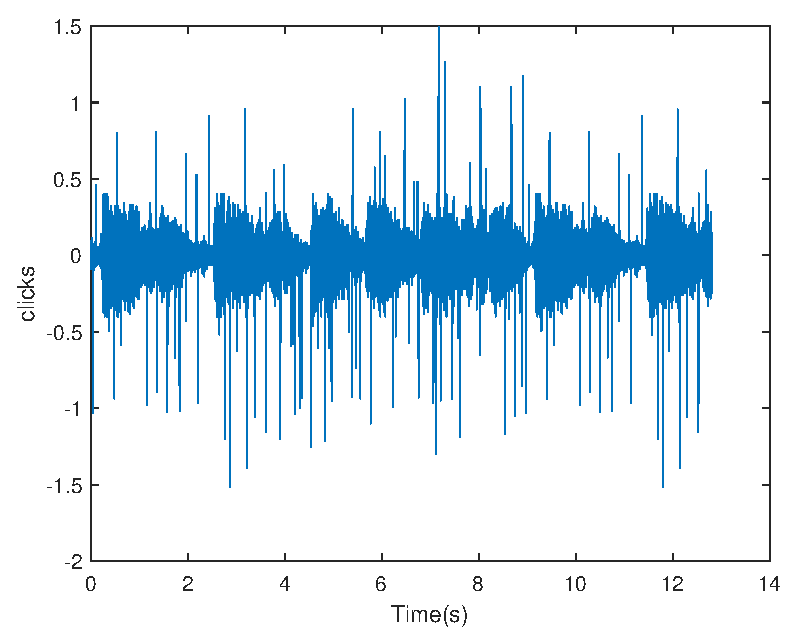
\includegraphics[width=6cm]{fig/fig1}
 		\caption{clicks in degraded signal}
 		\label{fig1}
 	\end{minipage}
 	\begin{minipage}[t]{0.48\textwidth}
 		\centering
 		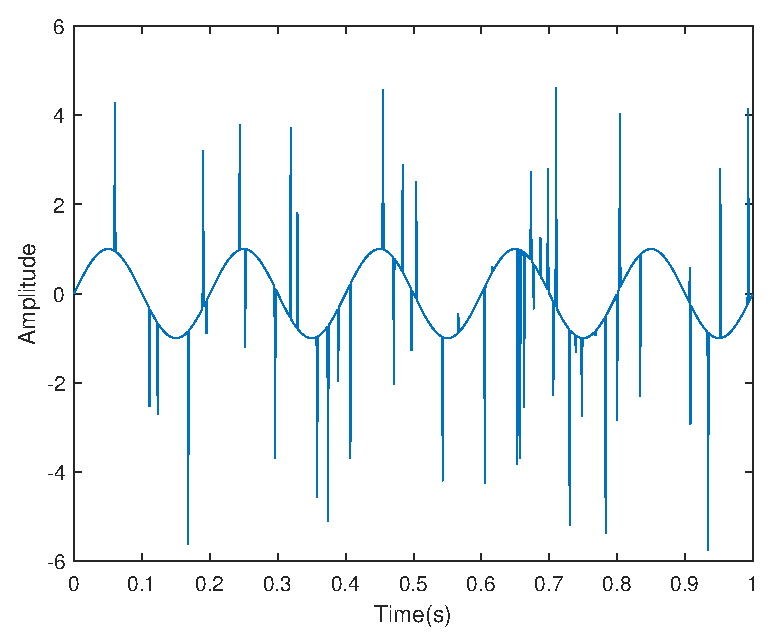
\includegraphics[width=6cm]{fig/fig2}
 		\caption{generated clicks}
 		\label{fig2}
 	\end{minipage}
\end{figure}
 
 
 \subsection{Detection}
We assume that we could detect the noise in the voice by using AR model. Hence we generate the AR model to predict the voice waveform and find the residual between original signal between them. With the error we found. We could set a threshold to judge if the data point is not reliable.
 
 \subsection{Interpolation}
 Having discovered $b_k$ we now need to replace these signal with the prediction. Again following our lectures we can use the AR model to interpolate the missing samples. Given ${\bf a}$ is our vector of AR coefficients and ${\bf b_k}$ is our detection vector and ${\bf s_o}$ is our original signal. We can insert the prediction data of the corresponding points into the distorted data and get a new data waveform.
 

\section{The algorithm}
The mathematical framework above only applies if the signal is statistically homogeneous. real signals are not, so we instead process the signal in blocks. Our algorithm is then as below.
\begin{enumerate}
    \item For each analysis block we process the inner $N_a$ samples shown in Figure \ref{fig3}. The analysis block contains a prediction error block and overlap samples. The overlap samples could make the result blocks connected with each other more smoothly.
    \begin{figure}[h]
    	\centering
    	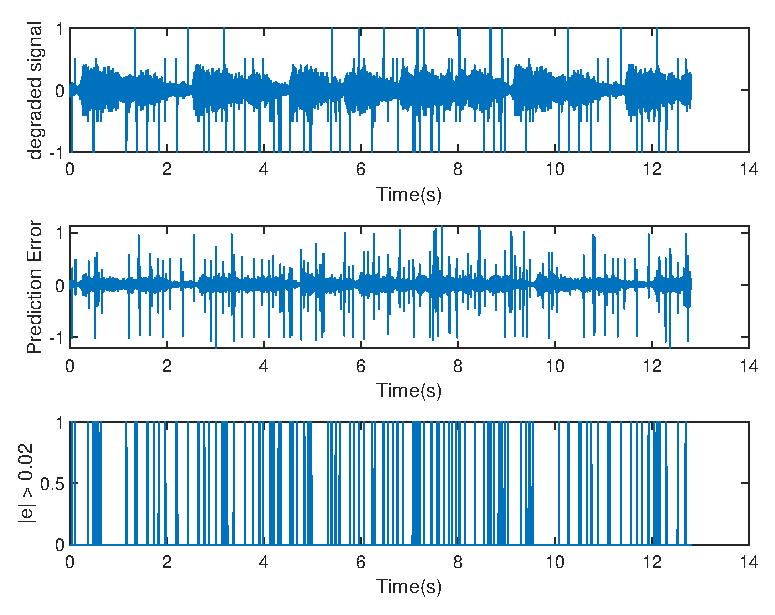
\includegraphics[width = .8\textwidth]{fig/fig3}
    	\caption{block-based processing}
    	\label{fig3}
    \end{figure} 
    \item Normalise the block by removing the dc level by making the mean value to 0.
    \item Estimate the AR coefficients of each analysis block.
    We can compute the coefficients of the AR model by using Normal Equations ~\ref{normalEquation}.
    
    \begin{equation}
    	a = R^{-1}r
    	\label{normalEquation}
    \end{equation}
    \item The residual of each sample $e_k$ is simply the difference between the actual signal sample $y_k$ and the prediction $\hat{y_k}$. Hence we can write ~\ref{residual}.
    
    \begin{equation}
    	e_k = y_k - \hat{y_k} = y_k - \sum_{p = 1}^{P} a_py_{k-p} = Ay = A_ky_k + A_uy_u
    	\label{residual}
    \end{equation}
    
    \item Threshold that error to give a detection indicator $b_k = (|e_k| > T)$ in each error block.
    \item With $b_k$, we want to interpolate predition value into the error location to correct the waveform. We can assume that the error ~\ref{residual} are 0 and hence solve for the missing data as follows ~\ref{equationofyu}.
    
    \begin{equation}
    	y_u = -{[A^{'}_{u}A_{u}]}^{-1}A^{'}_{u}A_{k}y_{k}
    	\label{equationofyu}
    \end{equation}
    
    \item Replace the missing data samples with these prediction value and assembly these data block together, finally we can get the final corrected signal.
    
\end{enumerate}



% An example of two figures side by side



\section{Experiments and results}
\subsection{Test with degraded artificial signal}
An artificial signal was generated using gaussian distributed random numbers filtered with an IIR filter which order is 3. Then the signal was artificially degraded by random clicks. Figure \ref{fig4} shows the ROC detection performance for different levels of degradation on this signal. We draw the scatterplot of TPR and FPR and fit. We found that the TPR/FPR level will increase with degradation level. As can be seen Figure \ref{fig5} shows that less level of noise, the model will perform better.

\begin{figure}[htbp]
	\centering
	\begin{minipage}[t]{0.48\textwidth}
		\centering
		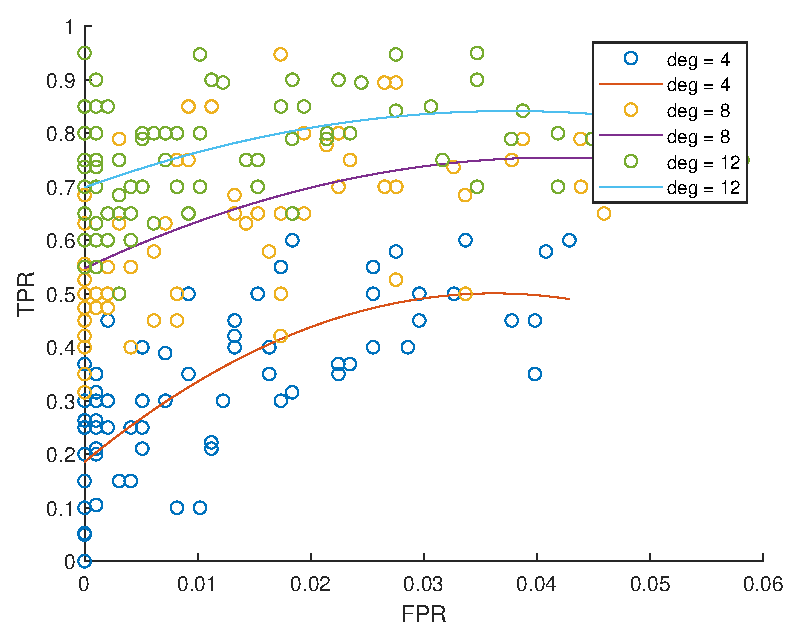
\includegraphics[width=6cm]{fig/fig4}
		\caption{TPR VS FPR(deg)}
		\label{fig4}
	\end{minipage}
	\begin{minipage}[t]{0.48\textwidth}
		\centering
		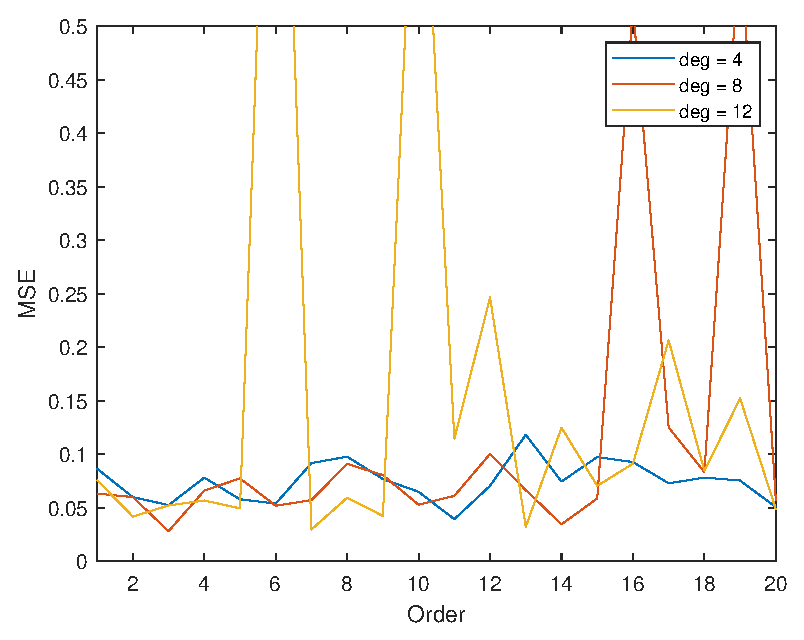
\includegraphics[width=6cm]{fig/fig5}
		\caption{MSE VS order(deg)}
		\label{fig5}
	\end{minipage}
\end{figure}

\subsection{Test with degraded clean signal}
A clean signal was then degraded using random amplitude and random location click noise. Figure \ref{fig6} and \ref{fig7} shows ROC results of the model with different p and bs. Figure \ref{fig8} shows the interpolation performance. We can find that higher order, block size will not lead to better performance absolutely. For example, TPR reachs to max value using p = 5. Thus we need to find out best parameters by assessing the performance of the model. Figure \ref{fig9} shows the output signal and the clicks are removed efficiently.

\begin{figure}[h]
	\centering
	\begin{minipage}{0.48\textwidth}
		\centering
		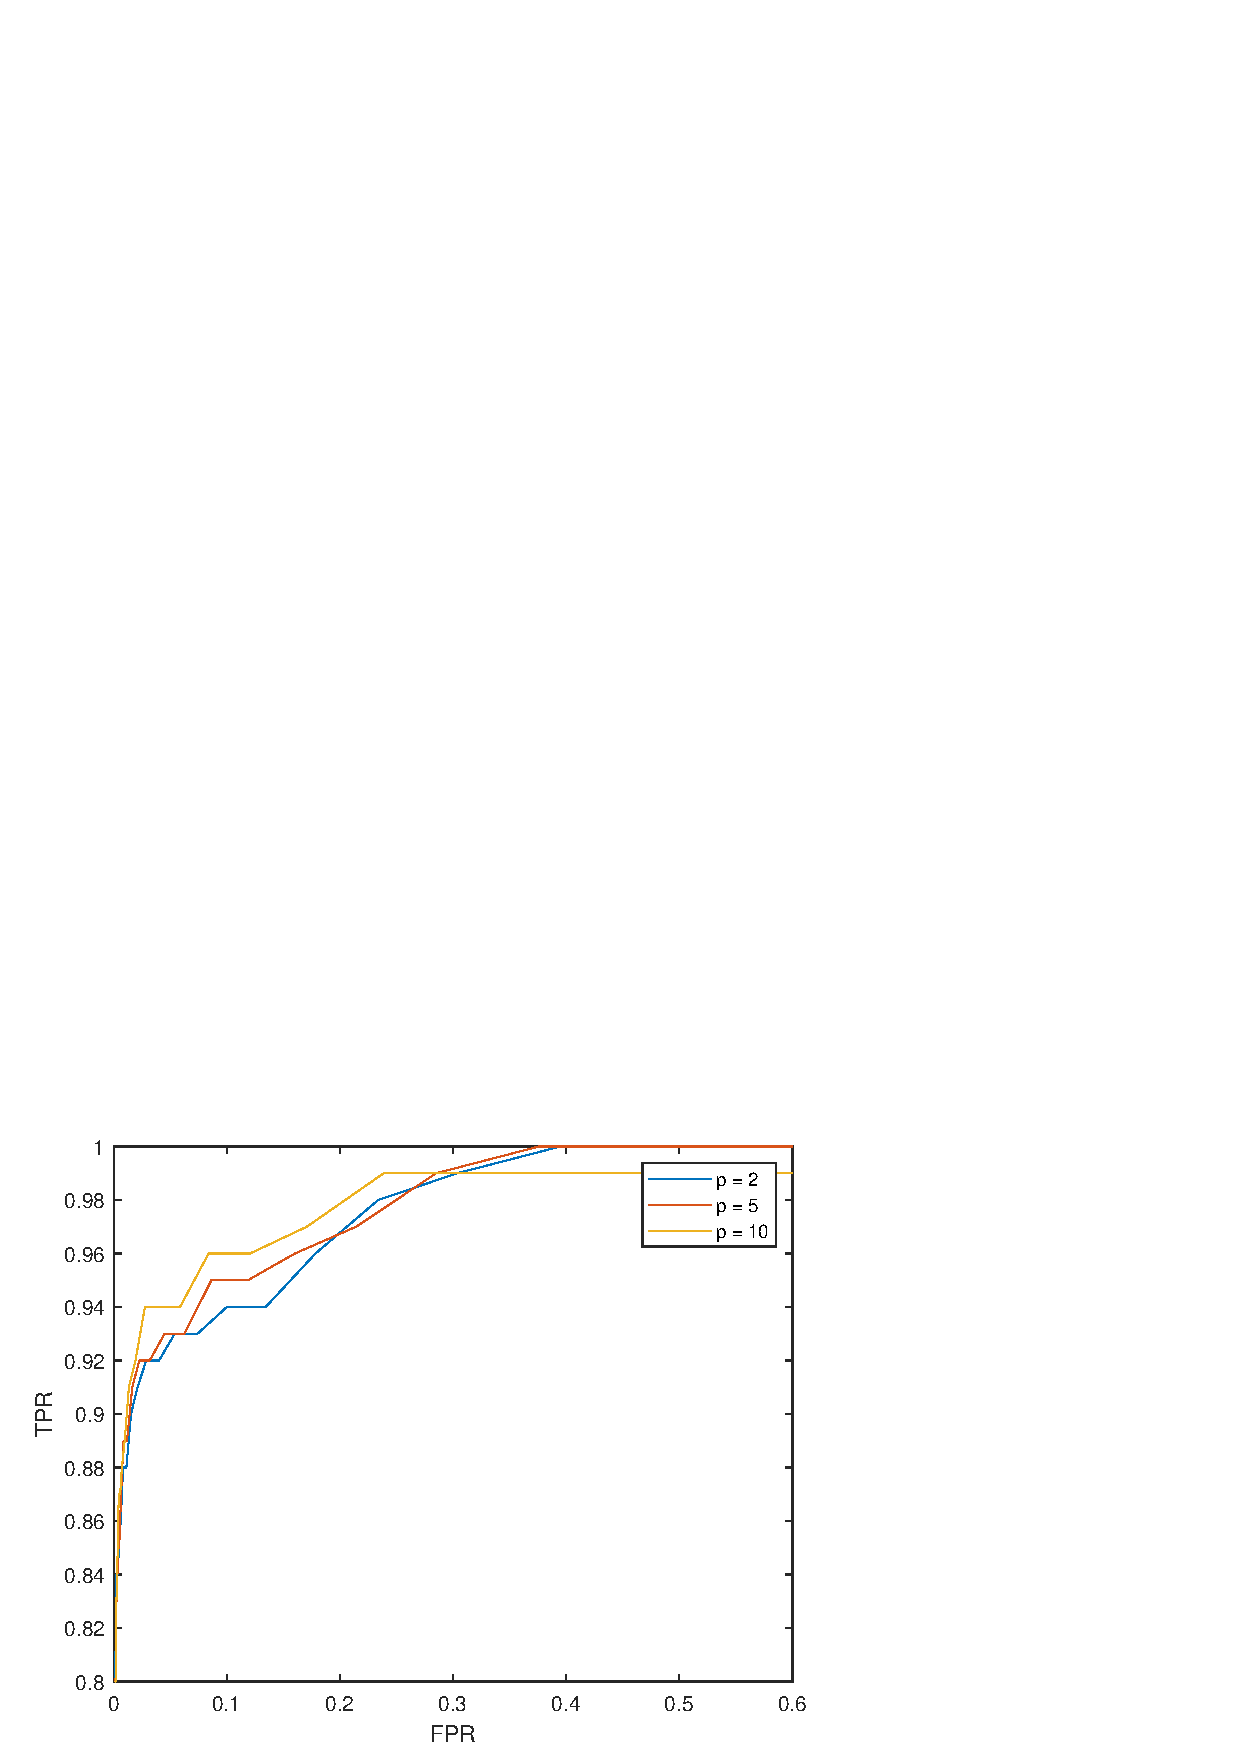
\includegraphics[width=6cm]{fig/fig6}
		\caption{TPR VS FPR (p)}
		\label{fig6}
	\end{minipage}
	\begin{minipage}{0.48\textwidth}
		\centering
		\includegraphics[width=6cm]{fig/fig7}
		\caption{TPR VS FPR (bs)}
		\label{fig7}
	\end{minipage}

\end{figure}
\begin{figure}[h]
	\centering

	\begin{minipage}{0.48\textwidth}
		\centering
		\includegraphics[width=6cm]{fig/fig8}
		\caption{MSE VS p(bs)}
		\label{fig8}
	\end{minipage}
	\begin{minipage}{0.48\textwidth}
		\centering
		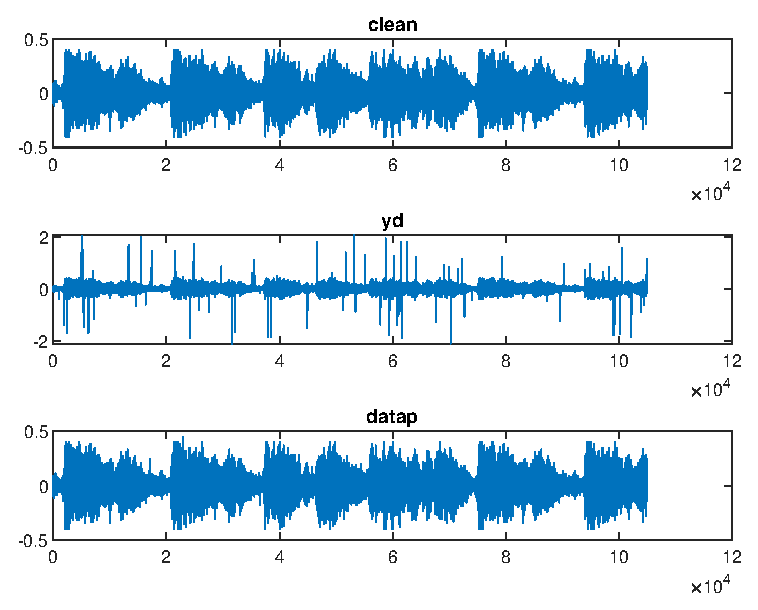
\includegraphics[width=6cm]{fig/fig9v2}
		\caption{compare signal}
		\label{fig9}
	\end{minipage}
\end{figure}


\subsection{Test with real signal}
To test on a real signal the original music was processed with given parameters and get results shown in table \ref{tab1}. The cleaned up signal is saved as restored.wav.\\
According to the method in previous, when the order is 6, we get max TPR/FPR as 1103, but inappropriate order will lead to the increase of max error.
When the block size is small, there will be more error. When the block size is larger than 1000, its performance is basically same, but it will have a impact on the running time.\\
Threshold will affect the detection performance. If it is small, the model will overpredict and deviate from the original signal; if it is too large, it will fail to find the point that should be corrected.\\
Proper overlap can reduce the max error and TPR/FPR.\\
According to the above methods, we have weighed the performance results and obtained the parameters as shown in Table \ref{tab1}.\\
The figure of exploring the relationship between parameters and performance is samiliar to the previous section. Due to space limitation, it will not be repeated here.\\

\begin{table}
	\centering
	\caption{parameters and results}
	\begin{tabular}{|c|c|c|c|c|c|c|}
		\hline
		parameter & order & block size & threshold & overlap & $b_k$ num & data size\\
		\hline
		value & 3 & 1200 & 0.35 & 2 & 134 & 105000\\
		\hline
		result & MSE & FPR(\%) & TPR(\%) & max error & TPR/FPR & run time\\
		\hline
		value & 0.000006 & 0.1 & 100 & 0.208 & 970.98 & 1.218\\
		\hline
	\end{tabular}
	\label{tab1}
\end{table}



\section{Conclusions}
This thing actually worked. But it was really hard to find best parameter for a model considering the efficiency, detection and interpolation performance. I wish we could have finished the performance assessment function first then it will save me much time. The interpolation function still have some problems that if we get very small coefficients in some cases, due to inverse operation in equation \ref{equationofyu}, it will lead $y_u$ to a large, impossible value. Maybe we could try other methods to acheive the interpolation or utilize threshold to avoid this case.


% Here are my references
%\bibliographystyle{acm}
%\bibliography{myrefs}

\end{document}
